%%%%%%%%%%%%%%%%%%%%%%%%%%%%%%%%%%%%

\section{1.5.Experimentos}

%%%%%%%%%%%%%%%%%%%%%%%%%%%%%%%%%%%%
\begin{frame}
\frametitle{Princípios do delineamento experimental}

\begin{enumerate}
\justifying
\item \hl{Controle:} Compare o tratamento de interesse a um grupo controle.
\justifying
\item \hl{Aleatoriedade:} Atribui-se aleatoriamente os elementos ao grupo controle e grupo tratamento, além disso a amostra também deve ser aleatória.
\justifying
\item \hl{Blocos:} Se houver variáveis que são conhecidas ou suspeitas de afetar a variável de resposta, primeiro agrupe os sujeitos em \hl {blocos} com base nessas variáveis e, em seguida, faça a randomização aos grupo tratamento e controle dentro de cada bloco.

\end{enumerate}

\end{frame}

%%%%%%%%%%%%%%%%%%%%%%%%%%%%%%%%%%%%

\begin{frame}
\frametitle{Mais sobre os blocos}


\twocol{0.25}{0.75}
{
\begin{center}
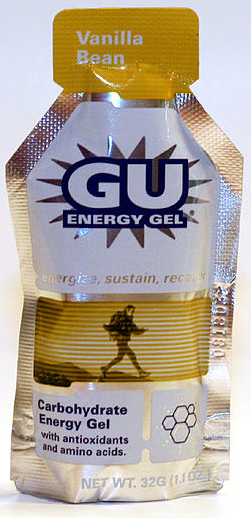
\includegraphics[width=\textwidth]{1-5_experiments/gu.png}
\end{center}
}
{
\begin{itemize}
\justifying
\item Gostaríamos de projetar um experimento para investigar se os géis de energia fazem você correr mais rápido:

\pause

\begin{itemize}
\item Tratamento: usar energy gel
\item Controle: não usar energy gel
\end{itemize}

\pause
\justifying
\item Suspeita-se que os géis de energia podem afetar os atletas profissionais e amadores de forma diferente, portanto, bloqueamos o status profissional:

\pause
\end{itemize}}
\end{frame}
%%%%%%%%%%%%%%%%%%%%%%%%%%%%%%%%%%%%

\begin{frame}
\frametitle{Mais sobre os blocos}

\begin{itemize}
   \begin{itemize}
   \justifying
\item Divida a amostra entre profissional e amador.
\justifying
\item Atribua aleatoriamente atletas profissionais a grupos de tratamento e controle.
\justifying
\item Atribua aleatoriamente atletas amadores para grupos de tratamento e controle.
\justifying
\item O status profissional/amador é igualmente representado nos grupos de tratamento e controle resultantes.
\end{itemize}
\end{itemize}


\pause

\dq{Por que isso é importante? Você pode pensar em outras variáveis para o bloco?}

\end{frame}

%%%%%%%%%%%%%%%%%%%%%%%%%%%%%%%%%%%%

\begin{frame}
\frametitle{Prática}
\justifying
\pq{Um estudo é projetado para testar o efeito do nível de luz e nível de ruído no desempenho de alunos em um exame. O pesquisador também acredita que os níveis de luz e ruído podem ter efeitos diferentes em homens e mulheres, portanto, quer garantir que ambos os gêneros estejam igualmente representados em cada grupo. Qual dos itens abaixo está correto?}
\small{
\begin{enumerate}[(a)]
\justifying
\item Existem 3 variáveis explicativas (luz, ruído, gênero) e 1 variável resposta (desempenho do exame).
\justifying
\solnMult{Existem 2 variáveis explicativas (luz e ruído), 1 variável de bloco (gênero) e 1 variável resposta (desempenho do exame)}
\justifying
\item Existe 1 variável explicativa (sexo) e 3 variáveis resposta (luz, ruído, desempenho do exame)
\justifying
\item Existem 2 variáveis de bloco (luz e ruído), 1 variável explicativa (sexo) e 1 variável de resposta (desempenho do exame)
\end{enumerate}
}
\end{frame}

%%%%%%%%%%%%%%%%%%%%%%%%%%%%%%%%%%%%

\begin{frame}
\frametitle{Diferença entre variáveis de bloqueio e explicativas}

\begin{itemize}
\justifying
\item Fatores são condições que podemos ser impostas nas unidades experimentais.
\justifying
\item As variáveis de bloqueio são características que as unidades experimentais têm e as quais gostaríamos de controlar.
\justifying
\item O bloqueio é como se fosse uma estratificação estratificação, exceto quando usado em configurações experimentais ao atribuir aleatoriamente, ao contrário de amostragem.

\end{itemize}

\end{frame}

%%%%%%%%%%%%%%%%%%%%%%%%%%%%%%%%%%%%

\begin{frame}
\frametitle{Mais terminologia de delineamento experimental ...}

\begin{itemize}
\justifying
\item \hl{Placebo:} tratamento falso, frequentemente usado como grupo de controle para estudos médicos.
\justifying
\item \hl{Efeito placebo:} unidades experimentais mostram melhora simplesmente porque acreditam que estão recebendo um tratamento especial.
\justifying
\item \hl{Cego:} quando as unidades experimentais não sabem se estão no grupo controle ou tratamento.
\justifying
\item \hl{Duplo-Cego:} quando tanto as unidades experimentais quanto os pesquisadores que interagem com os pacientes não sabem quem está no grupo controle e quem está no grupo tratamento.

\end{itemize}

\end{frame}

%%%%%%%%%%%%%%%%%%%%%%%%%%%%%%%%%%%%

\begin{frame}
\frametitle{Prática}
\justifying
\pq{Qual é a principal diferença entre estudos observacionais e experimentais?}

\begin{enumerate}[(a)]
\justifying
\item As experiências são realizadas em laboratório, enquanto os estudos observacionais não precisam de laboratório.
\justifying
\item Em um estudo observacional, observamos apenas o que aconteceu no passado.
\justifying
\solnMult{Estudos randomizados atribuem aleatoriamente os elementos ao grupo controle e ao grupo tratamento, enquanto os estudos observacionais não.}
\justifying
\item Estudos observacionais são completamente inúteis, uma vez que nenhuma inferência causal pode ser feita com base em seus achados.
\end{enumerate}

\end{frame}

%%%%%%%%%%%%%%%%%%%%%%%%%%%%%%%%%%%%

